\documentclass[DM,authoryear,toc]{lsstdoc}
% lsstdoc documentation: https://lsst-texmf.lsst.io/lsstdoc.html
\input{meta}

% Package imports go here.

% Local commands go here.

%If you want glossaries
%\input{aglossary.tex}
%\makeglossaries

\title{Second data facilities workshop findings}

% Optional subtitle
% \setDocSubtitle{A subtitle}

\author{%
William O'Mullane
}

\setDocRef{RTN-031}
\setDocUpstreamLocation{\url{https://github.com/lsst/rtn-031}}

\date{\vcsDate}

% Optional: name of the document's curator
% \setDocCurator{The Curator of this Document}

\setDocAbstract{%
After the data facilities workshop there were many interesting findings and issues. We have tried to capture them here.
}

% Change history defined here.
% Order: oldest first.
% Fields: VERSION, DATE, DESCRIPTION, OWNER NAME.
% See LPM-51 for version number policy.
\setDocChangeRecord{%
  \addtohist{1}{YYYY-MM-DD}{Unreleased.}{William O'Mullane}
}


\begin{document}

% Create the title page.
%\maketitle
% Frequently for a technote we do not want a title page  uncomment this to remove the title page and changelog.
\mkshorttitle to remove the extra pages

\section{Introduction}

The second data facilities workshop was held in 2022, Jan 19 and 20.
A series of presentations and discussions lead to very useful findings and actions.
See confluence for the slides etc. \url{https://confluence.lsstcorp.org/pages/viewpage.action?pageId=175440708}


This document is logically broken into area which emerged in the workshop and summarizes the discussions and some of the takeaways.

\section{Timeline}


\begin{itemize}
\item ComCam will go on the TMA next month
	\begin{itemize}
	\item We will have images, potentially on Sky images, before year end.
	\item We will have loads of calibration data
	\end{itemize}
\item We should be able to process ComCam images at SLAC in June.
	\begin{itemize}
	\item Would be nice to process all the BOT data
	\end{itemize}
\item Officially engineering first light is Jan 2023 (likely a little later)
	\begin{itemize}
	\item Then we need OGA racks etc.
	\item We will still be getting lots of engineering data from the real camera !
	\end{itemize}
\end{itemize}

The USDF timeline is in \citeds{RTN-021} the high level milestone chart is duplicated in\figref{fig:usdfplan} here.


\begin{figure}
\begin{centering}
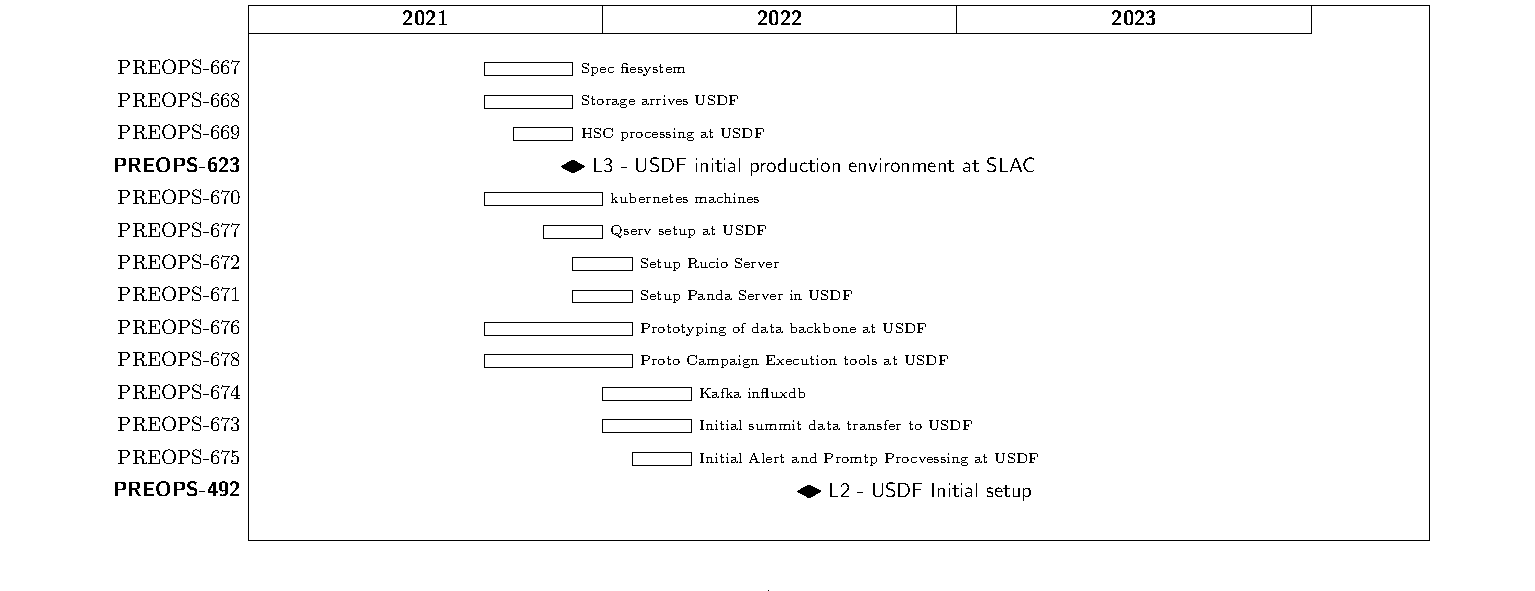
\includegraphics[width=0.9\textwidth]{USDFplan}
	\caption{USDF buildup plan from \citeds{RTN-021}\label{fig:usdfplan}}
\end{centering}
\end{figure}

The big question right now is {\em When can we start multi site testing with PanDA/Rucio ..
IDF, SLAC, FRdF all run PanDA \ldots}.

We need to build up tests for distributed processing RUCIO PanDA, which has started!


We need to make Jira Epics and capture decisions in technotes.

As always KISS!\footnote{Yes it is in the glossary.}



\section{Storage} 

\section{Processing} 

\section{Data movement} 

\section{Monitoring} 

\section{Conclusion}

This was a great workshop.
Nice to see a DM construction product, the pipelines,  used by the USDF execution team to process data.
There were a lot of good and practical solutions arrived at for DP0.2.
Now we need to scale that up for DR1 and of course do  DP1 and 2 on the way !


\appendix
% Include all the relevant bib files.
% https://lsst-texmf.lsst.io/lsstdoc.html#bibliographies
\section{References} \label{sec:bib}
\renewcommand{\refname}{} % Suppress default Bibliography section
\bibliography{local,lsst,lsst-dm,refs_ads,refs,books}

% Make sure lsst-texmf/bin/generateAcronyms.py is in your path
\section{Acronyms} \label{sec:acronyms}
\addtocounter{table}{-1}
\begin{longtable}{p{0.145\textwidth}p{0.8\textwidth}}\hline
\textbf{Acronym} & \textbf{Description}  \\\hline

DM & Data Management \\\hline
RTN & Rubin Technical Note \\\hline
\end{longtable}

% If you want glossary uncomment below -- comment out the two lines above
%\printglossaries





\end{document}
